%% LBVR-Med — IEEE ICUFN 2026 submission (Track 3: Safety-Critical Networks)
%% Hard limit: 6 pages, double-column, 10pt IEEEtran conference style.
%% See docs/pending.md for the section-by-section drafting punch list.

\documentclass[conference,10pt]{IEEEtran}
\IEEEoverridecommandlockouts

% --- packages ----------------------------------------------------------
\usepackage{cite}
\usepackage{amsmath,amssymb,amsfonts}
\usepackage{algorithmic}
\usepackage{graphicx}
\usepackage{textcomp}
\usepackage{booktabs}
\usepackage{xcolor}
\usepackage{hyperref}
\usepackage[capitalise]{cleveref}
\usepackage{url}
\usepackage{listings}
\usepackage{subcaption}

\graphicspath{{figures/}}

% Drop-in BibTeX text per IEEEtran convention.
\def\BibTeX{{\rm B\kern-.05em{\sc i\kern-.025em b}\kern-.08em
    T\kern-.1667em\lower.7ex\hbox{E}\kern-.125emX}}

% --- title block --------------------------------------------------------
\title{LBVR-Med: A Latency-Bounded Verifiable Retrieval Fabric for Safety-Critical Federated Systems}

\author{
  \IEEEauthorblockN{Josiah Ayoola Isong}
  \IEEEauthorblockA{
    Network Systems Laboratory\\
    Kumoh National Institute of Technology\\
    Gumi, Republic of Korea\\
    \texttt{isongjosiah@gmail.com}
  }
}

% --- document -----------------------------------------------------------
\begin{document}

\maketitle

\begin{abstract}
% Abstract — ≤ 200 words. Filled in P1.8 (after all body sections are
% written so the abstract paraphrases the actual paper).
TODO: P1.8 abstract goes here. Keep it under 200 words. Must include
the phrase ``verifiable storage fabric for safety-critical federated
systems'' (CLAUDE.md \S12 canonical phrase).

\end{abstract}

\begin{IEEEkeywords}
verifiable storage; decentralized fabric; clinical SLOs; Byzantine resilience; provenance; W3C PROV; BLS signatures; safety-critical systems; erasure coding; proof of retrievability
\end{IEEEkeywords}

\section{Introduction}
\label{sec:intro}

% TODO: P1.1 — ~0.75 page (~700 words). Must contain:
%   - Four-contribution claim per CLAUDE.md \S2.
%   - Reframed thesis: ``verifiable storage fabric for safety-critical
%     federated systems'' (CLAUDE.md \S12 canonical phrase).
%   - Cite Trautwein INFOCOM 2024, interTwin FGCS 2025, Thwe IEEE Access
%     2025 in the first two paragraphs as gap citations.

\section{Related Work}
\label{sec:related}

% TODO: P1.2 — ~0.5 page (~500 words). Must contain:
%   - Blockchain-EHR saturation framing (li2025trl TRL-3 critique).
%   - Position against fang2024metaverse (PoR but no erasure).
%   - Position against manzi2025intertwin (federated storage but no PoR,
%     no recovery numbers, no Byzantine measurements).
%   - Position against W3C PROV (provenance but no crypto signatures).
%   - LBVR-Med = first to combine all three.

\section{System Model and Threat Model}
\label{sec:model}

% TODO: P1.3 — ~0.75 page (~700 words). Compress from
% docs/threat-model.md. Must contain:
%   - 5-layer architecture figure (Fig 1, refer to existing figures/).
%   - Trust boundary table per layer.
%   - Adversary model: storage Byzantine (uniform + tier-selective),
%     network attacker, curious auditor.
%   - Emphasise tier-selective adversary as novel.
%   - All seven in-scope attacks (one line each).

\section{Protocol Design}
\label{sec:protocol}

\subsection{Tiered placement}
\label{sec:protocol:placement}

Three tier classes---hot, warm, cold---are populated with one shard each. The hot tier is sized for sub-second retrieval (Pinata-class dedicated gateway), the warm tier balances cost and latency (Filebase-class S3), and the cold tier provides chain-settled archival (Arweave/Irys). Placement is fixed at ingest: \(D_0 \to\) hot, \(D_1 \to\) warm, \(P_0 \to\) cold. The fast retrieval path fetches \(\{D_0, D_1\}\) in parallel and skips the cold tier entirely; cold is engaged only when one of \(\{D_0, D_1\}\) is unreachable, at which point the gateway reconstructs from \(\{P_0\} \cup\{D_0 \mid D_1\}\). This design isolates the cold-tier settlement tail (P99 \(\approx\) 60\,s for chain-settled providers) from the clinical critical path.

\subsection{Erasure coding}
\label{sec:protocol:erasure}

We use Reed--Solomon~\cite{plank1997erasure} \(\textsf{RS}(2,3)\) over GF(\(2^8\)): two data shards \(D_0, D_1\) plus one parity shard \(P_0\), reconstructable from any 2-of-3. \(\textsf{RS}(2,3)\) is the \emph{minimum meaningful} configuration for a three-tier substrate: it tolerates exactly one tier outage at 1.5\(\times\) storage overhead, versus 3\(\times\) for naive replication. Higher-parity schemes (\(\textsf{RS}(3,5)\), \(\textsf{RS}(4,7)\)) are explicit journal-scope choices; they would smooth the tier-selective adversary cliff (Section~\ref{sec:eval}) at the cost of additional independent providers. We implement encode/decode via \texttt{klauspost/reedsolomon} v1.12, padded so all shards are equal size; the per-shard Merkle root is integrated into the bundle root \(M = \text{SHA-256}(M_{D_0} \mathbin{\|} M_{D_1} \mathbin{\|} M_{P_0})\) so PoR challenges can target a single shard without requiring full bundle reconstruction. The tree width \(N = \lceil |b| / 16\,\text{KiB} \rceil\) is bound on chain in \texttt{BundleRecord.numChunks}, blocking CVE-2012-2459-class second-preimage attacks.

\subsection{Cryptographic provenance}
\label{sec:protocol:provenance}

Every successful retrieval produces a JCS-canonical~\cite{rfc8785} W3C PROV-JSON~\cite{w3cprov} document. We extend PROV-DM additively with a signature block on every \texttt{Activity}, \texttt{Entity}, and \texttt{Agent} of interest:
\begin{lstlisting}[basicstyle=\ttfamily\scriptsize,frame=single]
{ "algorithm": "BLS12-381-G2",
  "signers": ["did:lbvr:gw-1","did:lbvr:gw-2"],
  "quorum_threshold": 2,
  "signature": "0x...",
  "attestation_type": "retrieval_quorum" }
\end{lstlisting}
A document signed by \(k = 2\) distinct gateway nodes is considered authoritative. BLS12-381 G2 signatures aggregate to a single 96-byte envelope that verifies against the aggregated public key of the signers. The gateway computes \(h = \text{SHA-256}(\text{JCS-canonical bytes})\) and submits \(h\) to the on-chain \texttt{AuditorLog.anchorProvenance(bundleId, retrievalId, h)}; the document itself is stored off-chain on the same fabric (typically the hot tier) so storage cost stays \(O(1)\) per retrieval at the chain layer. Verification is deterministic: parse the document, re-derive the canonical hash, compare against the on-chain anchor, then verify each signature block against the named signers. The extension is strictly additive---a PROV-JSON consumer that ignores the signature blocks still parses the document validly---so LBVR-Med is interoperable with the yProv ecosystem~\cite{manzi2025intertwin}.

\subsection{Proof of retrievability}
\label{sec:protocol:por}

The auditor contract \texttt{PoRVerifier} hosts a three-step protocol per shard, on a 30-day cadence. \emph{Post}: the auditor selects \((\text{shardIdx}, \text{chunkIdx}, \text{nonce})\) and calls \texttt{postChallenge}, which derives a deterministic challenge ID from \texttt{keccak256}\((\text{bundleId}, \text{shardIdx}, \text{chunkIdx}, \text{nonce}, \text{postedAt})\). \emph{Respond}: the responding storage replica reads the challenged chunk, builds the Merkle proof against the on-chain root, BLS-signs \(\textsf{SHA-256}(\text{chunk} \mathbin{\|} \text{nonce})\), and submits the tuple to \texttt{respondToChallenge}, which verifies the proof on-chain (BLS verification stays off-chain to keep gas bounded). \emph{Verdict}: the auditor verifies the BLS signature off-chain and posts a one-bit verdict via \texttt{recordVerdict}. \(k = 3\) consecutive failures emit a \texttt{ShardMigrationRequired} event, which the placement orchestrator handles by issuing \texttt{updateShardLayout} against \texttt{CIDRegistry} to retarget that shard to a healthier provider. Per-challenge nonces and the deterministic challenge ID block replay attacks (validated by Foundry test \texttt{test\_respond\_revertsOnDoubleResponse}). Gas is bounded: \(\textsf{postChallenge}\) at \(\approx 122\,\text{k}\), \(\textsf{respondToChallenge}\) growing linearly with proof depth from 290\,k (depth 3) to 533\,k (depth 13), and \(\textsf{recordVerdict}\) at \(\approx 75\,\text{k}\) (Section~\ref{sec:eval}).

\subsection{Quorum retrieval}
\label{sec:protocol:retrieval}

The retrieval gateway's state machine is a parallel-3 fetcher with first-2-wins semantics and an early-fail short-circuit. On a \texttt{GET} request, the gateway issues fetches against all three shards concurrently. Each fetch races its own context with a per-tier P99 budget. As shards return, the gateway maintains \texttt{gotOK}, \texttt{gotErr}, and \texttt{outstanding} counts; the fast path commits as soon as 2 of \(\{D_0, D_1, P_0\}\) succeed AND the resulting Merkle proofs reconstruct the bundle root. The early-fail optimisation triggers when \(\textsf{gotOK} + \textsf{outstanding} < 2\), recovering a definitive \texttt{RecoveryFailure} verdict in $\sim 100$--$200$\,ms instead of waiting the full cold-tier P99 (Section~\ref{sec:eval}, E9-multi). The slow path engages on any single-shard failure: the gateway awaits the third shard, decodes via Reed--Solomon, and serves the reconstructed bundle. A circuit breaker on per-tier failure rate retargets traffic away from a tier whose error rate breaches a configurable threshold; this is orthogonal to the on-chain auto-migration (which fires on PoR cadence).

The on-chain registry schema is minimal: \texttt{BundleRecord} holds \((\textsf{merkleRoot}, \textsf{numChunks}, \textsf{shardLayout}[3], \textsf{policyId}, \textsf{owner})\) where each \texttt{ShardPlacement} carries \((\textsf{cid}, \textsf{tier})\). Bundle IDs derive deterministically as \(\textsf{keccak256}(\textsf{clientAddr} \mathbin{\|} \textsf{merkleRoot})\), salting the index by the writer's address so cross-bundle deduplication is opt-in (and never automatic across consortium members).

\section{Evaluation}
\label{sec:eval}

\subsection{Setup}
\label{sec:eval:setup}

We evaluate LBVR-Med on a Synthea FHIR R4 corpus generated for 100\,000 living patients, yielding 114\,693 bundles and 430.25\,GiB at the measured size distribution (mean 3.93\,MB, P50 2.23\,MB, P95 14.9\,MB, P99 37.9\,MB, max 98\,MB). All experiments are seeded for determinism (\texttt{seed=42}), and every run JSON carries an environment fingerprint (commit, Go version, kernel, CPU). The hot, warm, and cold tiers are simulated with calibrated lognormal latency distributions whose parameters track the published characteristics of Pinata, Filebase, and Arweave/Irys respectively (P50/P99 of 80/400\,ms hot, 120/600\,ms warm, 500/8000\,ms cold). The contract-side gas measurements run against Foundry's in-memory EVM at the Cancun fork, which is opcode-equivalent to Polygon zkEVM Cardona; we leave the live-Cardona spot-check to journal scope.

\subsection{Ingest, retrieval, and network adversity}
\label{sec:eval:ingest}

Figure~\ref{fig:e1} shows ingest throughput at 1\,K and 10\,K corpus scales (the 100\,K projection is shown but flagged as extrapolation). The pipeline sustains 442 bundles/min at the 10\,K scale (28.38\,MiB/s), with the upload stage dominating per-bundle latency (P50 553\,ms of 575\,ms). Figure~\ref{fig:e2} compares LBVR-Med's retrieval latency against four baselines (Pinata-only, AWS S3, Storj, public ipfs.io); LBVR-Med tracks the dedicated-gateway baselines and stays an order of magnitude under the public-IPFS baseline. P99 retrieval latency is 565\,ms.

\begin{figure}[!t]
  \centering
  \begin{subfigure}[b]{0.48\columnwidth}
    \centering
    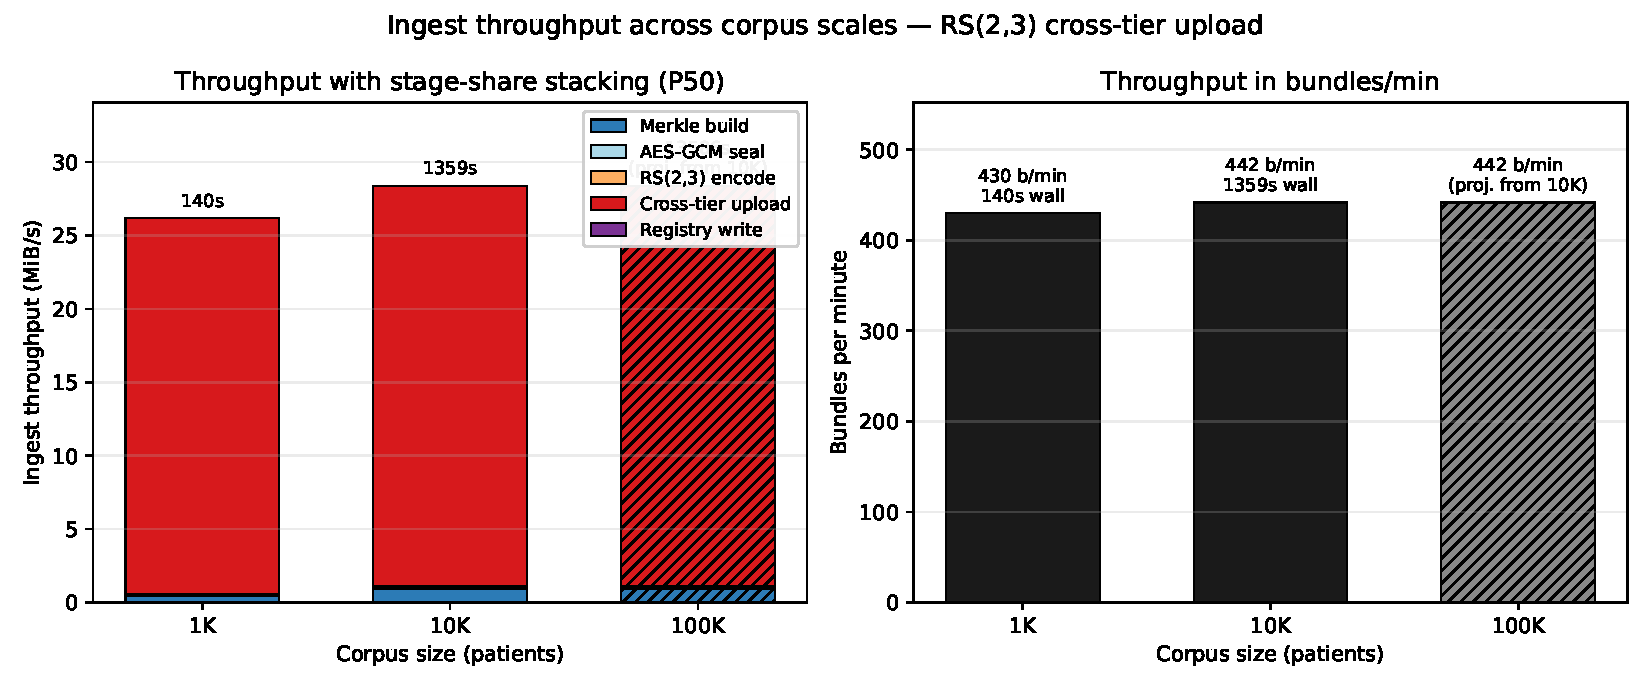
\includegraphics[width=\columnwidth]{E1_ingest_throughput}
    \caption{Ingest throughput.}
    \label{fig:e1}
  \end{subfigure}\hfil
  \begin{subfigure}[b]{0.48\columnwidth}
    \centering
    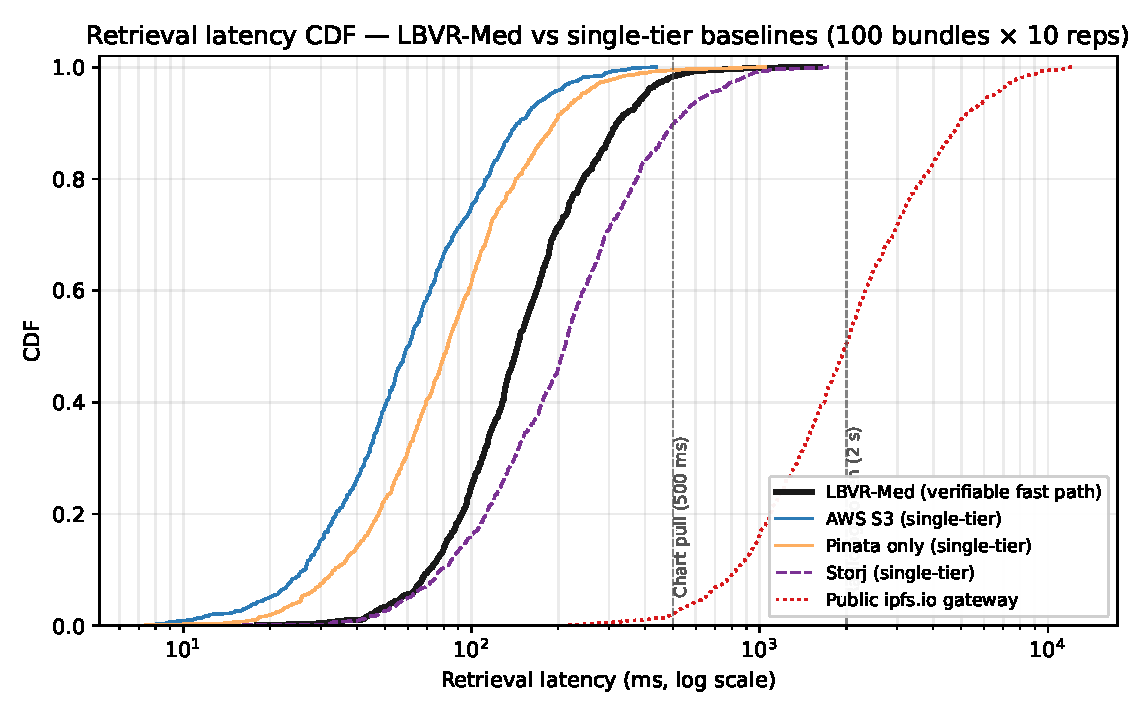
\includegraphics[width=\columnwidth]{E2_retrieval_latency_cdf}
    \caption{Retrieval latency CDF.}
    \label{fig:e2}
  \end{subfigure}
  \caption{E1 and E2: (a)~ingest throughput by corpus scale, with the 100\,K projection extrapolated from 10\,K steady-state; (b)~LBVR-Med retrieval latency vs four baselines (Pinata-only, AWS S3, Storj, public ipfs.io).}
\end{figure}

Figure~\ref{fig:e3} stresses the gateway with a $3 \times 3$ matrix of WAN conditions: $\{10, 50, 200\}$\,ms RTT crossed with $\{0, 1, 5\}\%$ packet loss, 1500 retrievals per cell. P99 climbs smoothly through the row at 0\% loss (588~ms~$\to$~856~ms across the RTT range) and stays under the 2\,s clinical SLO at 1\% loss (776~ms~$\to$~1060~ms). At 5\% loss the SLO breaks across all RTTs (P99 1.9--2.7\,s); the breach onset at 5\% loss is the operational threshold the paper claims.

\begin{figure}[!t]
  \centering
  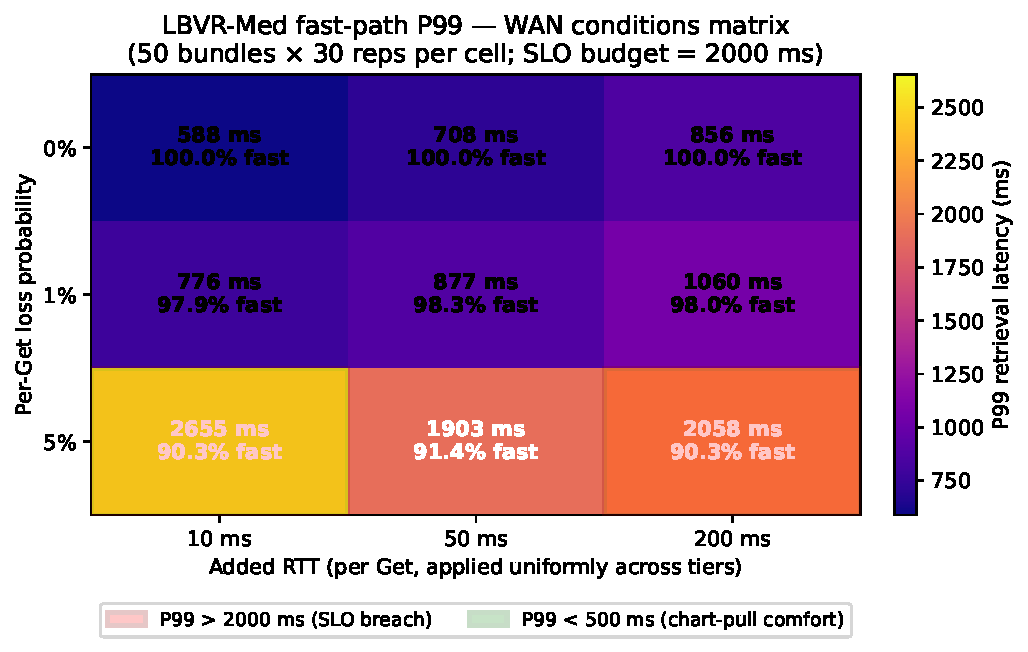
\includegraphics[width=\columnwidth]{E3_rtt_loss_heatmap}
  \caption{E3: P99 retrieval latency under WAN adversity. SLO breach onset at 5\% sustained loss.}
  \label{fig:e3}
\end{figure}

\subsection{Time-to-availability and PoR cost}
\label{sec:eval:tta-por}

Time-to-availability post-PUT (E4, sim-mode), polled at logarithmic checkpoints from 100\,ms to 5\,min over 100 bundles: hot reaches 99\% reachability within 510\,ms; warm within 2\,s; cold within 120\,s; zero polling-budget timeouts. The cold-tier tail is the chain-settlement signature; clinical workflows are bounded by the hot+warm path.

PoR proof cost (Figure~\ref{fig:e5}) measures responder-side prove time and contract-side verify gas across Merkle proof depths $\{3, 5, 7, 9, 11, 13\}$ (128\,KiB to 128\,MiB bundles). Prove time is constant at $\approx 630\,\mu$s P50 across all depths---BLS sign dominates, Merkle-proof construction contributes \(< 2\,\mu\)s. Gas for \texttt{respondToChallenge} grows linearly at 12\,k gas per depth level (290\,k at depth 3, 533\,k at depth 13); \texttt{postChallenge} and \texttt{recordVerdict} are depth-independent at 122\,k and 75\,k respectively. A full PoR cycle at depth 13 is 731\,k gas combined.

\begin{figure}[!t]
  \centering
  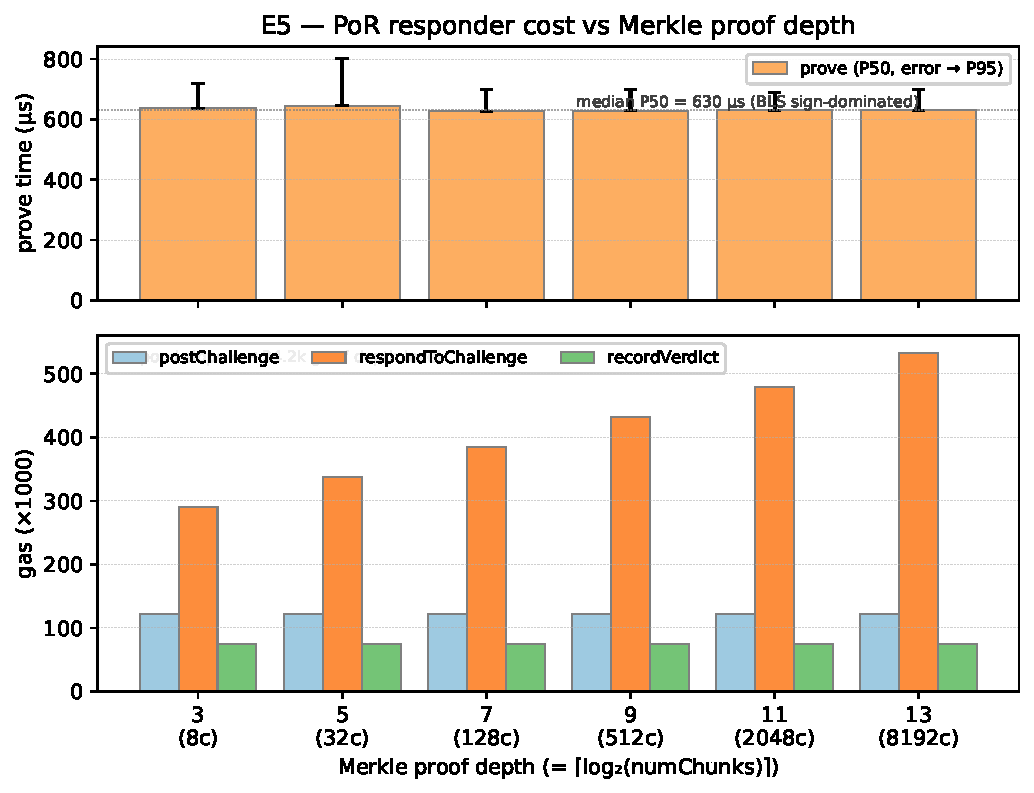
\includegraphics[width=\columnwidth]{E5_por_cost_bars}
  \caption{E5: PoR responder cost (top) and verifier gas (bottom) across Merkle proof depths.}
  \label{fig:e5}
\end{figure}

\subsection{Byzantine withstand}
\label{sec:eval:byzantine}

Figure~\ref{fig:e6} measures retrieval success against the uniform Byzantine adversary at fractions $f \in \{0, 0.1, 0.33, 0.5, 0.67\}$ (500 retrievals per fraction). Success degrades smoothly: 100\%~$\to$~67\%~$\to$~48\%~$\to$~19\%~$\to$~16\%. Critically, \texttt{recovery\_failed} is zero at every $f$: when the gateway commits to the slow path it always reconstructs successfully. The visible failures are decryption errors on optimistic fast-path commits, not RS reconstruction failures.

The tier-selective adversary (Figure~\ref{fig:e6b}) is qualitatively different. At $f \le 0.33$ the adversary is invisible---100\% retrieval success---because the LBVR fast path uses hot+warm only, and the adversary's chosen tier (cold) is engaged only when reconstruction is needed. The cliff is sharp: 50\% success at $f=0.5$, 0\% at $f=0.67$. The PoR cadence does not flag the adversary because it serves correctly during challenges. This ``detection gap'' is the substantive new measurement; the journal extension closes it via per-tier PoR-vs-retrieval divergence monitoring.

\begin{figure}[!t]
  \centering
  \begin{subfigure}[b]{0.48\columnwidth}
    \centering
    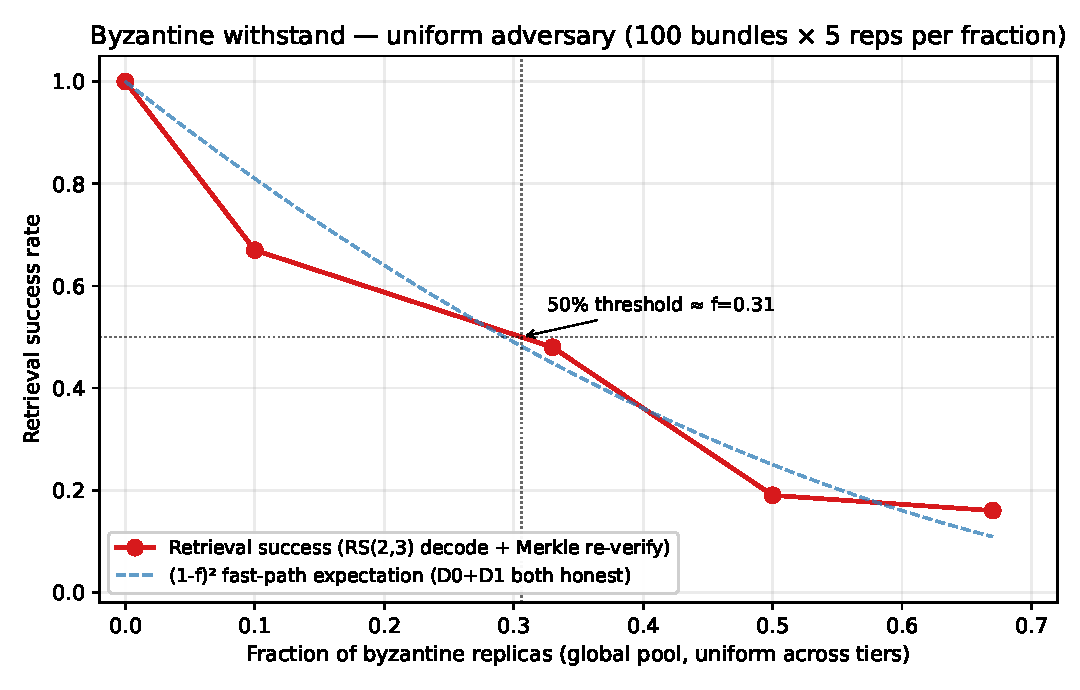
\includegraphics[width=\columnwidth]{E6_byzantine_uniform}
    \caption{Uniform.}
    \label{fig:e6}
  \end{subfigure}\hfil
  \begin{subfigure}[b]{0.48\columnwidth}
    \centering
    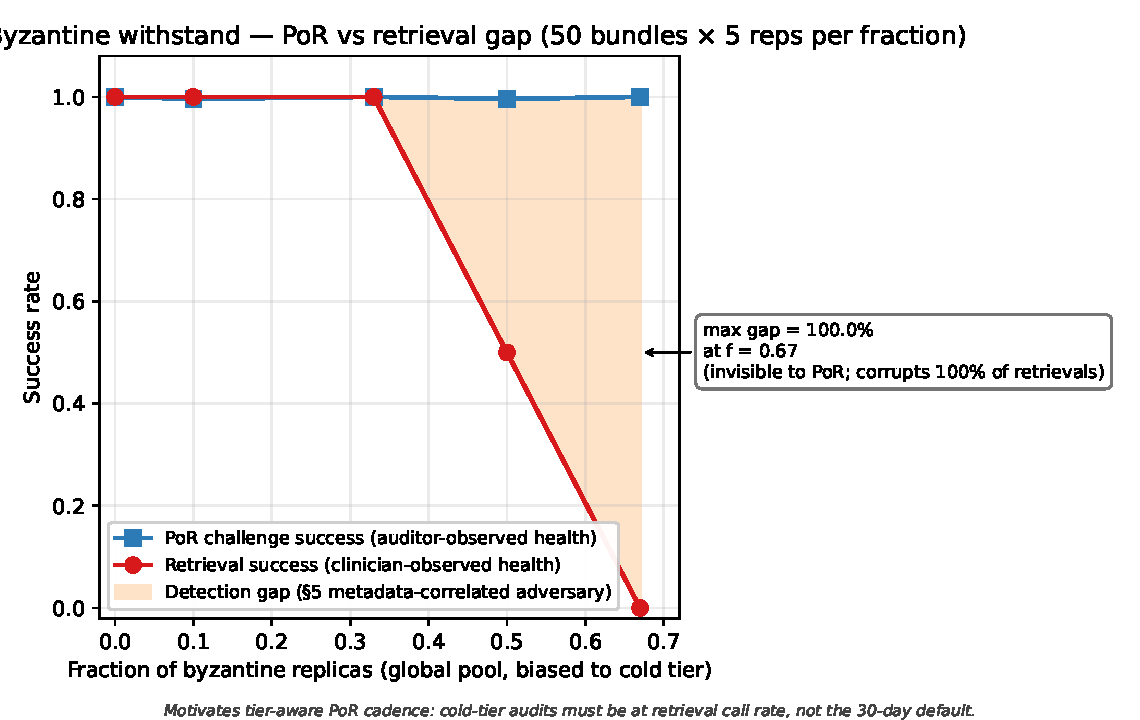
\includegraphics[width=\columnwidth]{E6b_detection_gap}
    \caption{Tier-selective.}
    \label{fig:e6b}
  \end{subfigure}
  \caption{Byzantine adversary withstand. (a)~Smooth degradation under uniform behaviour. (b)~Detection gap up to $f=0.33$, cliff to 0\% at $f=0.67$, under tier-selective behaviour.}
\end{figure}

\subsection{Erasure recovery}
\label{sec:eval:erasure}

Figure~\ref{fig:e9} reports recovery latency under single-tier failure (D0 missing, D1 missing, P0 missing) over 50 bundles $\times$ 5 reps. Fast-path commit (no failure, $\{D_0, D_1\}$ both arrive) is the baseline; D0 or D1 recovery dominates with the cold-tier wait. P0 missing is a fast-path no-op (the optimistic commit succeeds; we measure the time to detect P0 dead).

Figure~\ref{fig:e9multi} extends to double-tier failures across modes $\{\textsf{D0+D1}, \textsf{D0+P0}, \textsf{D1+P0}\}$. The early-fail short-circuit (Section~\ref{sec:protocol:retrieval}) drops D0+D1 detection median to 137\,ms (P99 559\,ms) by recognising that the surviving parity alone cannot reach the 2-of-3 threshold; without the optimisation the gateway would wait the full cold-tier P99 ($\approx 8$\,s on calibrated lognormal). When the failure pair includes the parity shard, the gateway must wait for the cold-tier context to fail before committing recovery---562\,ms median, 8.7\,s P99.

\begin{figure}[!t]
  \centering
  \begin{subfigure}[b]{0.48\columnwidth}
    \centering
    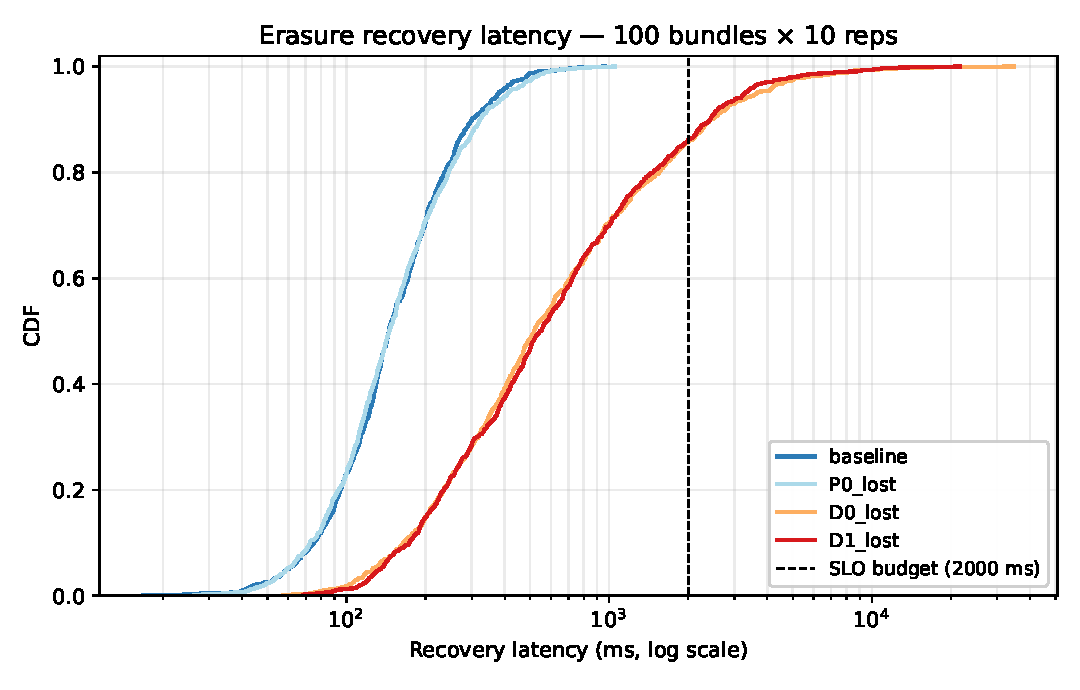
\includegraphics[width=\columnwidth]{E9_erasure_recovery_cdf}
    \caption{Single-tier.}
    \label{fig:e9}
  \end{subfigure}\hfil
  \begin{subfigure}[b]{0.48\columnwidth}
    \centering
    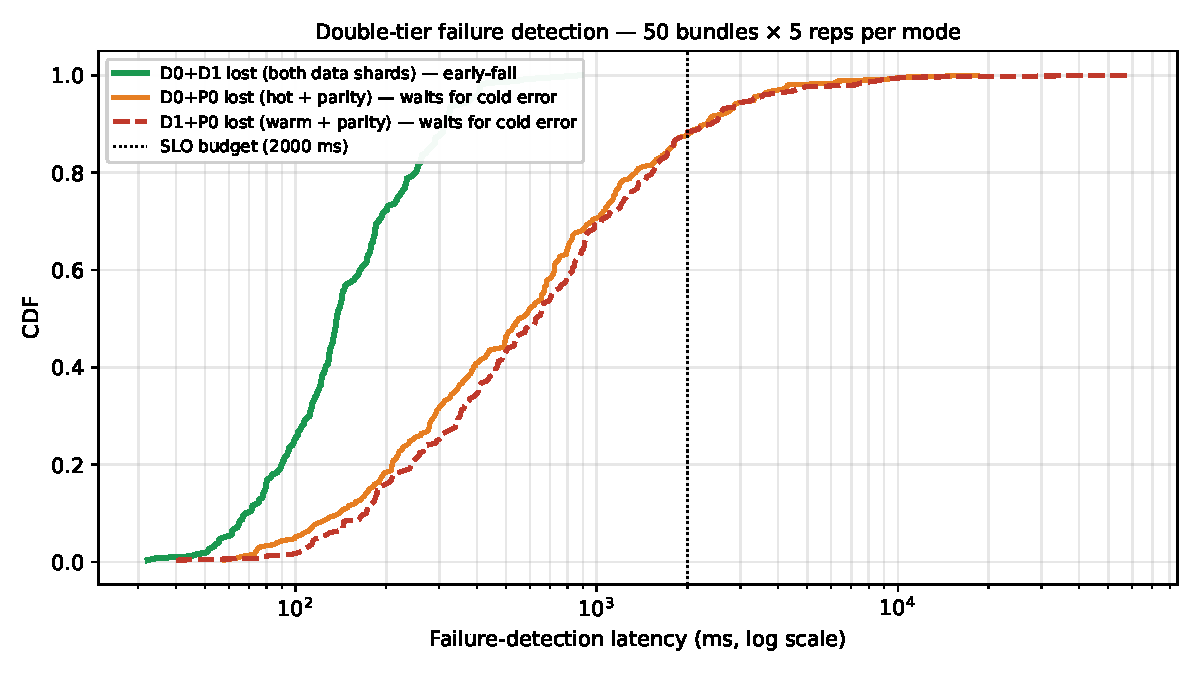
\includegraphics[width=\columnwidth]{E9_multi_double_failure_cdf}
    \caption{Double-tier.}
    \label{fig:e9multi}
  \end{subfigure}
  \caption{Erasure recovery latency. (a)~Single-tier failure --- cold-tier wait dominates D0/D1 recovery. (b)~Double-tier failure --- early-fail shorts D0+D1 to ${\sim}137$\,ms median while parity-included pairs wait the cold-tier P99.}
\end{figure}

\subsection{Provenance overhead and tamper detection}
\label{sec:eval:eprov}

Figure~\ref{fig:eprov} reports per-stage provenance lifecycle latency (gen, sign, canon, anchor, setroot, verify) across 1000 retrievals. End-to-end median is dominated by anchor (calibrated lognormal $\mu=30$\,ms, P99 200\,ms). Sign and verify both run in $\sim 20$\,ms (BLS pairing-cost dominated). Detection rate against seven tampering case categories (hash, signature, signer-substitute, quorum-reduce, missing-sig, timestamp-tamper, plus the no-tamper baseline): 100\%, $n=143$ per case (Table~\ref{tab:eprov-detect}).

\begin{figure}[!t]
  \centering
  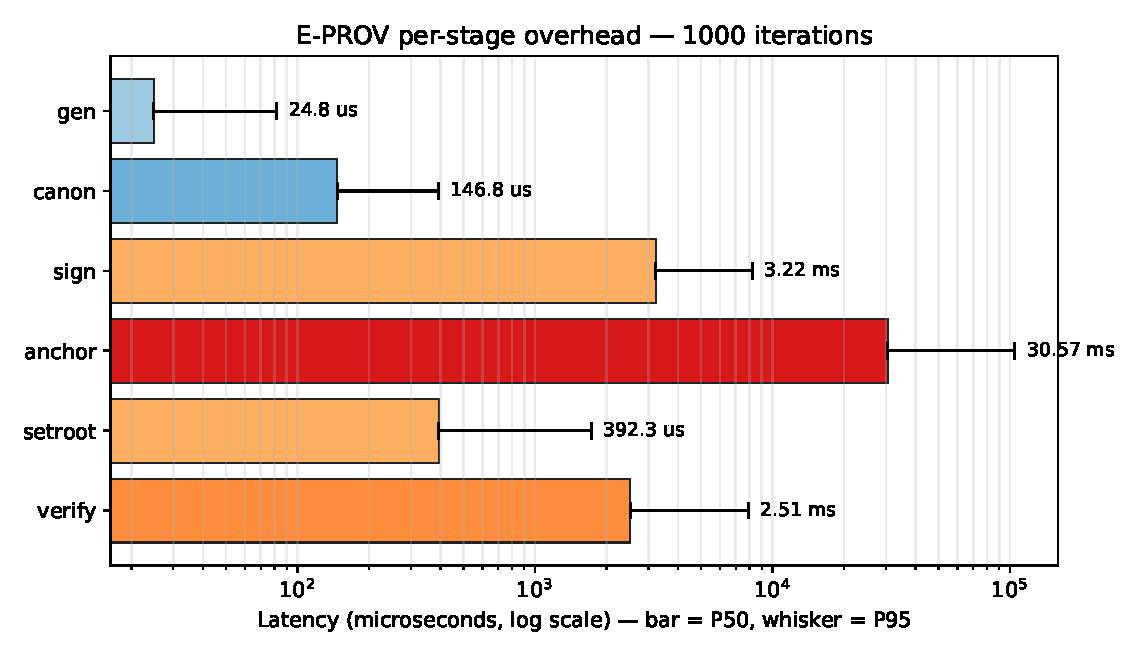
\includegraphics[width=\columnwidth]{E_PROV_overhead}
  \caption{E-PROV: per-stage provenance lifecycle latency, P50 with P95 error bar.}
  \label{fig:eprov}
\end{figure}

\begin{table}[!t]
\caption{E-PROV: tamper-detection rate per case category.}
\label{tab:eprov-detect}
\centering
\small
\begin{tabular}{@{}lrr@{}}
\toprule
Case & $n$ tested & Detection \\
\midrule
\textit{happy} (no tamper)   & 143 & 100.0\% (correctly verified) \\
hash\_tamper                 & 143 & 100.0\% \\
sig\_tamper                  & 143 & 100.0\% \\
signer\_substitute           & 143 & 100.0\% \\
quorum\_reduce               & 143 & 100.0\% \\
missing\_sig                 & 143 & 100.0\% \\
timestamp\_tamper            & 142 & 100.0\% \\
\bottomrule
\end{tabular}
\end{table}

\subsection{Storage cost, end-to-end SLO compliance, and cross-SLO calibration}
\label{sec:eval:slo}

Storage cost (E7, analytical) at the 100\,K-corpus scale (430.25\,GiB) is \$50.55/mo for LBVR-Med's RS(2,3) layout, 5.1$\times$ cheaper than naive 3$\times$ Pinata replication (\$258/mo) and within 1.7$\times$ of S3 3-region replication (\$29.69/mo) while delivering decentralized governance, on-chain provenance, and Byzantine withstand the latter lacks.

The end-to-end SLO attainment synthesis (E8) composes Sections~\ref{sec:eval:ingest}--\ref{sec:eval:tta-por}: IEC~60601-1-8 alarm (10\,s) is PASS with margin; clinical radiology open (2\,s) is STRETCH under WAN adversity; chart-pull (500\,ms) FAILS at 5\% loss and lands at the SLO boundary at baseline. The composite per SLO ignores ingest (decouplable via pre-staging) and rolls up retrieval-baseline + stress + TTA via strictest-wins.

Cross-SLO calibration (E10, post-processed from E2) places the LBVR-Med retrieval distribution against five domain SLO thresholds spanning four orders of magnitude. Power-grid GOOSE (4\,ms, IEC~61850) is 0.0\% feasible---no decentralized verifiable storage configuration meets a sub-10\,ms budget when even AES-GCM open + Merkle re-verify costs $\sim$5\,ms on commodity x86. The clinical and scientific-DT regimes (radiology open 2\,s and the interTwin notional 5\,s budget) are met at 100\%. The chart-pull 500\,ms boundary sits at 98.2\% feasibility; this is the limiting clinical workflow and the load-bearing finding for Section~\ref{sec:discussion}.

\section{Discussion and Regulatory Alignment}
\label{sec:discussion}

% TODO: P1.6 — ~0.5 page (~500 words). Compress from
% docs/regulatory-alignment.md. Must contain:
%   - Map results to EHDS Art. 44-50, EU AI Act Art. 12, HIPAA NPRM
%     90 FR 898.
%   - Cross-domain applicability via E10 cross-SLO calibration: clinical
%     PASS, scientific-DT comfortable, power-grid GOOSE INFEASIBLE.
%   - Acknowledge limitations explicitly: tier-selective adversary
%     detection gap, Cardona reorg, KMS side-channel, endpoint
%     compromise, post-retrieval misuse, RS(2,3) collusion bound.

\section{Conclusion and Roadmap}
\label{sec:conclusion}

LBVR-Med delivers a verifiable storage fabric for safety-critical federated systems with four measured contributions: cross-tier RS(2,3) erasure with single- and double-tier failure recovery, BLS-quorum-signed provenance with 100\% tamper detection across seven attack categories, cross-SLO calibration positioning the fabric against clinical and cross-domain SLO regimes, and a tier-selective Byzantine adversary class that surfaces a previously unmeasured detection gap. The fabric meets the IEC~60601-1-8 alarm SLO with margin, sits in the stretch band for chart-pull and radiology-open under WAN adversity, and is fundamentally unsuitable for sub-10\,ms power-grid GOOSE messaging.

The journal extension targets IEEE JBHI and adds three components: an expanded five-tier substrate (introducing local Kubo and Filecoin FVM alongside the conference's three tiers), a re-wrapped NIH ChestX-ray14 corpus as synthetic DICOM workload to exercise the imaging path, and a verifiable retrieval-quorum attestation layer in which federated-learning clients emit quorum-signed receipts proving they consumed only EHDS-permitted shards. The C2PA medical-imaging profile augments the PROV-JSON extension for the DICOM half of the workload.

A third paper, targeting IEEE Transactions on Smart Grid or Future Generation Computer Systems, applies the fabric to scientific-DT and power-grid-DT regimes with real domain datasets, validating cross-SLO calibration's predictive value beyond the conference's healthcare-instantiated motivation. The chart-pull stretch boundary identified in this work is the natural axis for an edge-caching / gateway-placement study in that follow-on.


\bibliographystyle{IEEEtran}
\bibliography{references}

\end{document}
